\subsection{FET}

\subsubsection{Calculo de los capacitores del amplificador}
Para hallar los valores de cada capacitor del amplificador anterior sección se
calculan los siguientes valores:

\begin{enumerate}
\item Frecuencia de corte para cada capacitor del amplificador:
\begin{equation*}
    \begin{split}
        f_{\text{c2}} &= 1[k\text{Hz}]\\
        f_{\text{c1}} &= 0.2\,f_{\text{c2}} = 200[\text{Hz}]\\
        f_{\text{c3}} &= 0.2\,f_{\text{c1}} = 40[\text{Hz}]\\
    \end{split}
\end{equation*}
\item Circuito RC de entrada:
\begin{equation*}
    C_1 = \frac{1}{2\pi\,(R_i + (R_1 || R_2))\,f_{\text{c1}}}
    = \frac{1}{2\pi(350[\Omega]+(\frac{(1000)(100)}{1000+100}))(200[\text{Hz}])}
    = 1.80485[\mu\text{F}]
\end{equation*}
\item Circuito RC de salida:
\begin{equation*}
    C_3 = \frac{1}{2\pi(R_i + (R_D + R_L))\,f_{\text{c3}}}
        = \frac{1}{2\pi(470[\Omega]+470[\Omega])(40[\text{Hz}])}
        = 4.23284[\mu\text{F}]
\end{equation*}
\item Circuito RC de puenteo:
\begin{equation*}
    \begin{split}
        R_{\text{eq}} &= R_S || (1/g_{\text{m}})
                       = \frac{(150)(1/0.024331)}{150+(1/0.024331)}
                       = 32.260[\Omega]\\
        C_2 &= \frac{1}{2\pi\,R_{\text{eq}}\,f_{\text{c2}}}
             = \dfrac{1}{2\pi\,(32.260[\Omega])(1000[\text{Hz}])}
             = 4.93343[\mu\text{F}]\\
    \end{split}
\end{equation*}
\end{enumerate}

\subsubsection{Simulación de computadora}
Se utilizó el software \emph{Quite Universal Circuit Simulator.} versión 23.3.1
para simular el circuito amplificador, este puede verse en la
\textbf{figura~\ref{figura24}}.

\begin{figure}[!h]
\centering
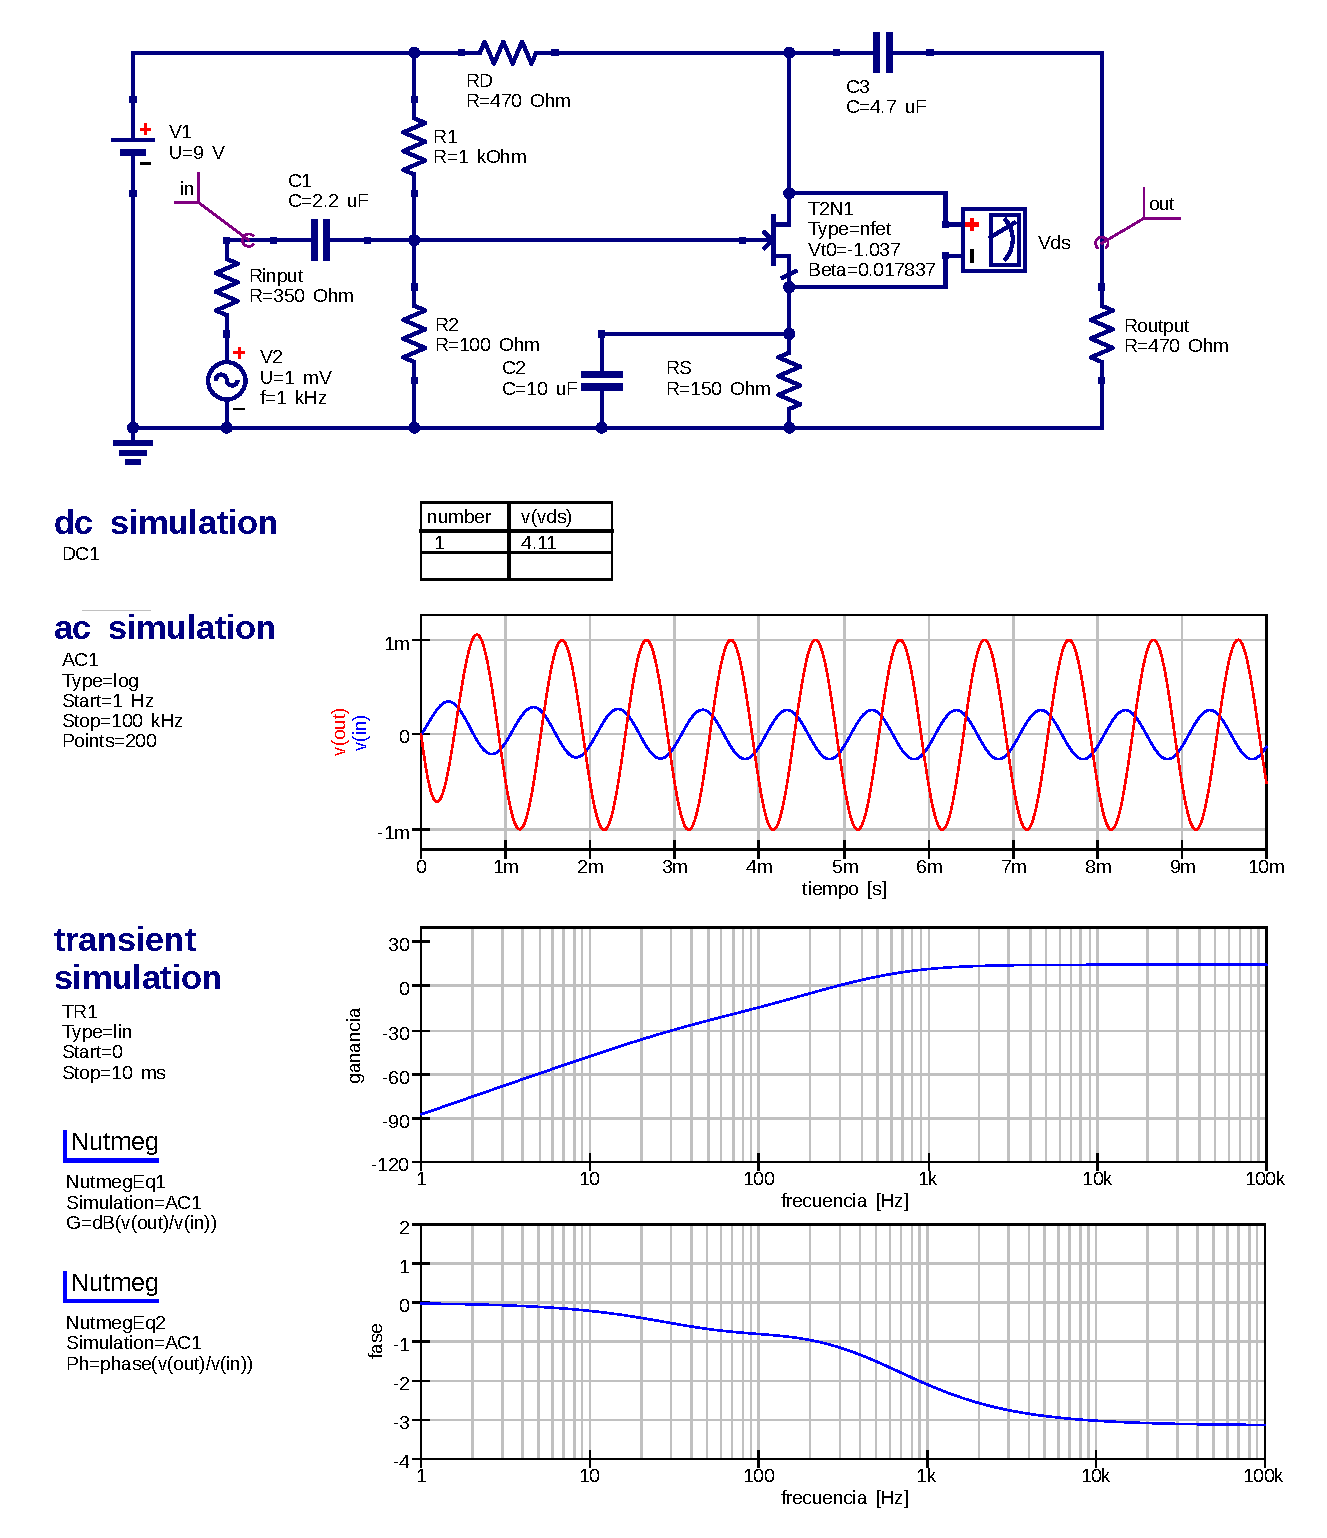
\includegraphics[scale=0.72]{diagramas/figura24.eps}
\caption{Simulación del amplificador.}
\label{figura24}
\end{figure}

